%\setcounter{page}{1}
\chapter{Introduction}\label{chp:intro}

Imagine you are given a mechanical duck. It quacks and moves awkwardly. At a certain point, you take it apart and study all the gears and pulleys that make it up, enabling you to understand how it works. By getting more ducks, you realize that all gathered together simply quack and walk like the first one. Nothing more. However, if you get your hands on a real bird, e.g.a starling, it is a completely different story. Instead of taking it apart (please do not), you observe it and eventually learn something about it, such as its diet and sleep patterns. But when you encounter a flock of starlings, you realize that studying a single bird does not prepare you for the emergent behavior of the group. The flock can create intricate patterns in flight, something that you would not have imagined from observing a single starling (Figure~\ref{fig:intro:duck}). \\

\begin{figure}[h]
    \centering
    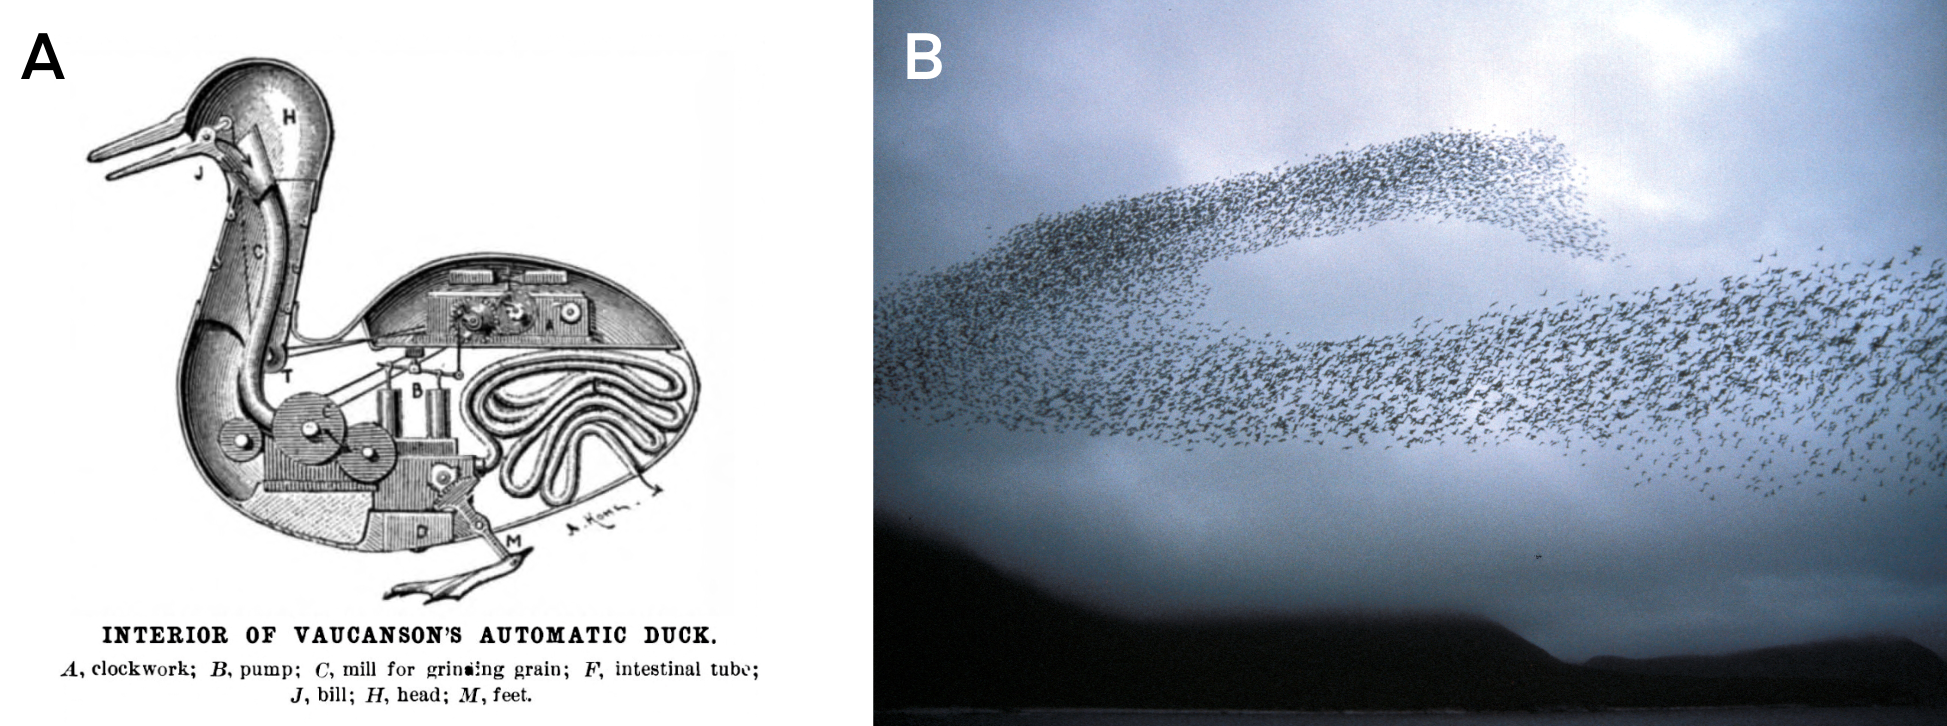
\includegraphics[width=\textwidth]{figures/intro/duck_flocking.png}
    \caption[Reductionism and emergence]{The digestive duck (Panel A) has become a symbol of reductionism, which states that the behavior of every system could be described as the sum of its individual components' contributions. A flock of birds, on the other hand, illustrates the concept of collective animal behavior (Panel B). It is considered an emergent behavior that arises from individuals following simple rules without any central coordinator. Images from Wikimedia Commons under public domain.}
    \label{fig:intro:duck}
\end{figure}

The philosophical attitude underneath the approach taken with the mechanical duck is called reductionism. It claims that systems can be explained by reducing them to their fundamental components. Reductionism has been highly successful in some scientific fields, especially in physics. However, this approach fails to explain all the rich behavior of some physical systems, such as the spontaneous symmetry breaking observed in many-body physics \cite{anderson1972more}. These systems exhibit irreducible properties at all scales that cannot be explained by studying their individual components alone, like the swarm behavior of a flock of starlings. Emergent phenomena are present also in other fields such as ecology and biology. For example, we find the formation of ant colonies (a population of ants capable of coordinating social and complex tasks without a central controller), the creation and maintenance of ecosystems (which are composed of a multitude of different interacting species), or the synchronization of fireflies. There are examples from a social standpoint too. The richness of human interactions is evidenced by viral information spreading, economic growth, or the evolution of language. \\

The ubiquity of emergent properties makes it apparent that many systems are more than the sum of their parts, and a classic approach does not work with them. As P. W. Anderson stated in this seminal 1972 paper \cite{anderson1972more}, ``the ability to reduce everything to simple fundamental laws does not imply the ability to start from those laws and reconstruct the universe''. It is at this point where complex systems science comes into play. Adopting an interdisciplinary approach, complexity science investigates how emergent properties arise and how they affect the behavior of the system as a whole. Drawing on concepts and tools from physics, mathematics, biology, and computer science, to name but a few, it aims to better understand the complexity of the world around us. However, despite the large number of systems we can claim to be complex, an operative definition of complex systems has been elusive. \\

The term's ambiguity should not cause concern \cite{horgan1995complexity}, since other crucial concepts still generate significant debate regarding their formal scientific definition. These concepts include consciousness, sustainability, and life. As with the elusive concept of life \cite{schrodinger1992life}, instead of attempting to provide a scientific definition of complexity, we will outline the essential characteristics of typical complex systems \cite{de2019complexity}. This will enable us to identify and differentiate them from systems that we might classify as very complicated, but not necessarily complex, such as the mechanical duck. As mentioned earlier, typical  complex systems exhibit emergence and self-organization, which happens when interactions between their (usually) many components produce a global pattern of behavior. These interactions are highly heterogeneous and may generate new information, making it challenging to study isolated components or accurately predict future outcomes. The unpredictable long-term behavior that complex systems display is often driven by their non-linear dynamics and the presence of phase transitions. Complex systems may adapt their interactions to changing environmental conditions, as opposed to merely approaching a steady state. Given the emphasis on interactions, it is not surprising that the main challenge of complexity science is to understand how the structure of these interactions gives rise to the system's behavior as a whole.\\

%Here, paragraph of why ecology and social science can be seen as complex systems:
Certainly, the characteristics of complexity discussed in the previous paragraph can be observed in a wide variety of situations, including natural and social systems. Natural ecosystems are considered paradigmatic examples of complex systems due to their adaptative power, presence of patterns, and their diversity of species and interactions. Precisely this remarkable biodiversity and heterogeneity make them a paradigmatic illustration of complexity. \cite{levin1998ecosystems}.  It is not surprising then that, in the young field of ecology \cite{ghazoul2020ecology}, complex systems' approaches have been taken to understand the functioning of species-rich communities. To gain these insights, ecosystems are often described as complex networks, rather than just individual pairwise interactions, to examine their structure and how it affects their dynamics. Depending on the research question, this network description can be done at several levels of organization: individual-based networks, followed by species-based, and finally, clade-based networks \cite{guimaraes2020structure}. Studying complex systems at different scales is important because it provides us with different perspectives on the system's behavior. Moreover, recent approaches at a macroscopic level have highlighted the presence of statistical patterns in community structure, which indicate the presence of fundamental principles or laws of nature \cite{brown1995macroecology,brown2004toward}. These patterns manifest as scaling relationships and recurrent distributions with similar parameters across different communities \cite{west1997general}. Exploring ecosystems as complex adaptive systems allows us to address some central questions, especially regarding the relationships between structure and functioning, the existence of universal biodiversity patterns, and the mechanisms that determine them \cite{levin1998ecosystems}.\\

% ECO   in coexistence: statisctical physics, random matrix theory and nonlinear dynamics . No decir todo el rato coexistence, tambien persistence
% social systems e interdiscipliplinariedad, paper Computational Social Science ≠ Computer Science + Social Data 

% SOCIAL: transportation airports... 
Complexity is pervasive in social phenomena as well.  A typical social system is composed of agents whose collective behavior is not usually manifested in the properties of the single constituents. For example, it would be inadequate to use the trajectory of one individual as the only reference to study mobility in a city, and as a case in point, a city itself is much more than the aggregation of its buildings and people. There are plenty of cases in which the lens of complex systems has deepened our understanding of human activity. In this context, the spreading of diseases has been a problem extensively addressed within the complex systems community, developing more and more complete models that integrate simultaneous processes \cite{soriano2018spreading}, and anticipate the advance of outbreaks \cite{mazzoli2023spatial}. Moreover, power grid fluctuations \cite{martinez2023dynamical}, pedestrian dynamics \cite{zuriguel2020contact} and the impact of road disruptions have been modeled to improve overall system performance \cite{bassolas2020scaling}. Lastly, in the context of social relationships,  large advances have been made towards explaining the arise of cooperation \cite{axelrod1981evolution}, which has been a major challenge in human behavior and other disciplines \cite{Nowak2006EvolutionaryDynamics}.\\

Ecological and social systems are just two examples among all the contexts that can be regarded as complex. Indeed, they appear in many scientific domains, and hence the traditional methodology of each domain is not enough to fully explore complex systems in a unified way. Instead, computational modeling and mathematical tools are required and developed to explore the structure and evolution of complex systems. Among these methods, two frameworks have proven extremely useful, which we will adopt in this thesis. One is that of complex networks, which connect the interactions’ architecture with the collective dynamics. For example, by describing the relationship between pollinators and plants as networks, it has been found that their nested structure increases species persistence and resilience \cite{cota2019echo}.  From a social perspective, the emergence of cooperation also depends on the connectivity of the network of connections \cite{raducha2022coordination}. Political polarization and the spread of diseases have also found a network description very profiting. Complex systems may have processes working at different spatial and temporal scales. Thus, the other perspective is that of looking at the systems from different scales to gain a complete understanding of the interplay of different processes. Ultimately, a macroscopic description of the systems can characterize and explain statistical patterns that span different orders of magnitude. In linguistics, for example, it is well-known Zipf’s law, which describes the word frequency distribution in the vast majority of linguistic corpora  \cite{zipf1999psycho}. Analogously, the metabolic rate of organisms varies as a power law with temperature and body size \cite{brown2004toward}, and, within social phenomena, the production of goods or consumption of energy scale nonlinearly as a function of city size \cite{west2017scale}. \\

Furthermore, studying complex systems at different scales allows us to understand the contribution of each level of description to the overall dynamics. Therefore, we will address our following challenges from different scales of description. By taking a more holistic approach to complex systems modeling, we can gain a better understanding of how various interactions influence one another and how emergent properties arise. This, in turn, can inform our understanding of real-world systems and help us to develop more accurate predictive models. \\

\section{Our contributions}
Despite significant advances in complex systems modeling, there is still much to explore. This thesis focuses on the challenges related to ecological interactions. Since there is a current trend to develop ecological models that capture the heterogeneity of these interactions, a complex systems approach is suitable for studying them. Then, the first goal of this thesis is to investigate how emergent properties, particularly the coexistence of multiple agents, are affected by the inclusion of space, several interactions simultaneously, and different interaction topologies. \\

%most of these models fail to capture all the heterogeneity of their interactions. Typically, these models consider only one type of interaction at a time, ignoring potential interdependencies between different types and the effects of time and space on them. In thesis, we aim to address these limitations by exploring how emergent properties, in particular the coexistence of many different agents, are affected by these considerations. \\

\subsection{Bridging ecological and social systems}\label{chp:intro:bridge}
 The versatility of the complexity paradigm allows it to address a wide range of problems across different contexts with a common language, borrowing concepts and models from different types of complex systems. We can adopt established solutions from other systems to tackle problems in our own settings. Specifically,  one can examine the similarities between ecological systems and human interactions in the context of online social networks (OSNs). They have revolutionized how we communicate and process information, but also have brought to light the cognitive limitations of our brains. We have gone from a situation where we only received information from a few broadcast sources to being inundated with millions of messages demanding our attention. As a result, there has been an acceleration of social dynamics \cite{lorenz2019accelerating}, and the concept of ``competition for attention'' has become commonplace. Furthermore, OSNs are designed to capture and retain our attention by providing instant gratification \cite{fareri2014social,malik2016gratification} and reinforcing feedback \cite{sherman2018brain}. These limitations, combined with the vast amount of information produced every second, have resulted in competition between ideas/memes for visibility, leading users to adopt various strategies to increase the likelihood that their messages will be read. \\

The strong emphasis on how competition shapes information communications and on how users respond to it has inspired researchers to draw an analogy between natural and social systems \cite{borge2017emergence,lorenz2019accelerating,palazzi2021ecological,plata2021neutral,calleja2021quantifying,tovo2021upscaling}. Actors (like users and memes) of OSNs are seen as species of ecological communities that aim to maximize their abundance --visibility for users, popularity for memes--, and that are competing for a limited resource: the individuals' attention. Furthermore, the communication strategies adopted by the users can be interpreted in ecological terms too: posting specific hashtags to provide context to users' messages can be represented as mutualism, as it favors both visibility of users and the growth of the involved hashtags. With this ecological bridge, we can depict OSNs as ``information ecosystems'' (Table~\ref{tab:bridge}).\\

\begin{table}[t]
\caption[Ecology-Social networks bridge]{Terminology equivalence for the ecological-social systems' bridge.}
\centering
\footnotesize
\begin{tabular}{cccc}
\hline
                    & \textbf{Population}   & \textbf{Variant}        & \textbf{Individual} \\ \hline \hline
\textbf{Macroecology}                & Community    & Species        & Organism   \\ \hline
\textbf{Microbial systems} & Sample       & OTU            & Read       \\ \hline
\textbf{Component systems}           & Realization  & Component      & Token      \\ \hline
\textbf{Online Social Networks}      & Bin & Meme, User  & Post   \\ \hline
\end{tabular} \label{tab:bridge}
\end{table}

This analogy has recently been applied to explain, for example, the acceleration of collective attention with a mathematical model based on Lotka-Volterra equations \cite{lorenz2019accelerating}. Alternately, the concept of ecological neutrality \cite{hubbell2001unified,azaele2016neutral} has also been used in more theoretical works, which were able to reproduce several macroscopic patterns found in online social networks \cite{plata2021neutral}. New insights on the functioning of information ecosystems have been the work of Borge-Holthoefer {\it et al.} \cite{borge2017emergence}, who studied the structure of online discussions of social protests as an ecological network, finding that its architecture became nested, in very close resemblance to the typical organization of natural mutualistic assemblages \cite{bascompte2003nested,bastolla2009mutualism}.\\

Moreover, while ecological theory is rich in models, collecting empirical data is often difficult due to limitations in time and resources. Conversely, social systems generate a vast amount of data that is easier to get and combine. The proposed analogy between natural and information ecosystems can open the doors for the application of ecologically-inspired models without being hindered by data availability. In fact, we could push the boundaries further and refine models for social systems that surpass the limitations imposed by ecological data. \\

The second goal of this thesis is to demonstrate the potential benefits of this ecological bridge to tackle social challenges. We will address the drivers that govern the coexistence of users and hashtags in online discussions and the emergent patterns that their dynamics creates. \\

\subsection{Structure of this thesis}
Following the analogy between ecological and social interactions presented in the previous Section, this thesis is divided into two parts. The first of them is dedicated to the drivers of coexistence in natural communities, which are conveniently described as complex networks. Traditionally, one of the first questions asked in ecological networks was about the structure of empirical real networks. Are there any commonalities among networks of the same type of interaction \cite{Fontaine2011TheNetworks}? Are these patterns conserved across different geographical locations \cite{galiana2022ecological}? It seems that while there are certain shared structural characteristics, they are not common to all interaction types. Some of these patterns are a heterogeneous degree distribution \cite{jordano2003invariant} and nested architecture \cite{bascompte2003nested}  if the interactions are positive for all the species involved. In competitive communities, it remains the fundamental question of whether the interactions form a hierarchy. \\

The study of ecological networks presents challenges that are not exclusive to the domains of ecology, like introducing space in present network models. Spatial connectivity and temporal patterns have a profound effect on the dynamics at several scales from populations to whole ecosystems \cite{intro2020theoretical}. In particular, space may play a critical role in promoting the coexistence of an array of different situations like competition for space  \cite{maynard2017diversity,godoy2017intransitivity, Dieckmann2000}. We dedicate Chapter~\ref{chp:1} to developing a simplified ecosystem where individuals of each species compete and lay on a spatial network. We consider intransitivity and locality of interactions since they are only possible between individuals at a certain distance. Varying such distances allows us to interpolate between local and global competition. We will check how stable coexistence can be achieved depending on the architecture of the interactions. \\

Moreover, as mentioned previously, empirical networks  have  traditionally  considered interactions in isolation, e.g. pollination \textit{or} competition for nectar. These studies suggest that single-interaction networks exhibit structural regularities. However, there is recent and increasing evidence (\cite{kefi2012more, kefi2016structured,dominguez2021structure, Garcia-Callejas2018ThePersistence, Garcia-Callejas2021TheConstraints}) that important ecological questions like resilience to perturbations and persistence of species also depend on the interplay between interactions of different nature. We will precisely follow this historical trend in Chapter~\ref{chp:2} to discover how the place species have in their interaction network affects their survival to extinction after a perturbation in interaction strengths, and how the importance of those structural properties changes if more interactions are considered simultaneously. At the end of the day, an ecological community is a complex system composed of several types of interactions and numerous species. Then, chances are that a reductionist approach, in which every interaction is studied in isolation, could not completely capture all the emergent behavior that the ecosystem presents. \\

We dedicate the second part of the thesis to the study of social systems, in particular, online social networks from an ecological perspective.  OSNs serve not only as platforms to build social connections but also as news sources. As a result, our communication model has shifted from our traditional centralized mass media outlets and face-to-face interactions to a new era where all actors are both information receivers and sources. This new paradigm has made OSNs an excellent example of social information processing, which leads to emergent phenomena like fake news spreading \cite{del2016spreading}, viral information  \cite{weng2013virality}, and the creation of echo chambers \cite{del2016echo, cota2019echo}.\\


%The strong emphasis on how competition shapes information communications and on how users respond to it has inspired researchers to draw an analogy between natural and information ecosystems \cite{borge2017emergence,lorenz2019accelerating,palazzi2021ecological,plata2021neutral,calleja2021quantifying,tovo2021upscaling}. Actors (like users and memes) of OSNs are seen as species of ecological communities that aim to maximize their abundance --visibility for users, popularity for memes--, and that are competing for a limited resource: the individuals' attention. Furthermore, the communication strategies adopted by the users can be interpreted in ecological terms too. For example, posting specific hashtags to provide context to users' messages can be represented as mutualism, as it favors both visibility of users and the growth of the involved hashtags. With this ecological bridge, we can depict OSNs as ``information ecosystems'' (Table~\ref{tab:bridge}).
Building on the aforementioned ecological-social bridge, in a recent study by Palazzi {\it et al.} \cite{palazzi2021ecological}, we proposed an ecology-inspired model \cite{suweis2013emergence,cai2021niches} to explain the structural flexibility displayed by OSNs when responding to external disturbances like breaking news. In Chapter~\ref{chp:3}, we develop a methodology to infer the interaction values of the ecologically-inspired model of that previous work. We study how these interactions change during exogenous events and test with empirical data whether visibility optimization can be the driver of those changes.  \\

Finally, in Chapter~\ref{chp:4}, we go to a much higher level of abstraction, leaving the particularities of the single agents or particular settings. We investigate the presence of scaling laws and abundance distributions in online social networks. To do that, we also rely on the ecological bridge to translate well-known macroecological patterns into the context of human communication. Like the heterogeneity of life, that spans several orders of magnitude, information ecosystems also reflect that variety in their size and temporal dynamics. The genome size varies from merely $10^4$ nucleotides in simple viruses to more than $10^{10}$ in some vertebrates and plants. Similarly, online discussions involve hundreds of posts to thousands and the number of followers that users accumulate, and hence their potential visibility, goes from $10^0$ to more than $10^8$. The presence of general patterns, common to different complex systems, potentially facilitates the identification of universal generative processes and functional constraints, making it easier to solve problems in a variety of contexts. For example, if a particular pattern is found to be common to both ecological systems and social communication, insights from one field could be applied to the other.

% The examples of ecological and social complex systems, despite the differences in the nature of their microscopic description, may exhibit similar complex behavior on the macroscopic scale. 